% Arquitectura de AlexNet (red convolucional profunda)
% Compilar con: pdflatex alexnet_architecture.tex
\documentclass[tikz,border=10pt]{standalone}
\usepackage{tikz}
\usepackage{amsmath}
\usetikzlibrary{arrows.meta}

\definecolor{gdlblue}{RGB}{41, 98, 168}
\definecolor{gdlred}{RGB}{191, 49, 49}
\definecolor{gdlgreen}{RGB}{30, 130, 76}
\definecolor{gdlorange}{RGB}{217, 130, 30}
\definecolor{gdlpurple}{RGB}{118, 56, 138}
\definecolor{gdlgray}{RGB}{140, 140, 140}
\definecolor{gdlyellow}{RGB}{190, 140, 10}

\begin{document}
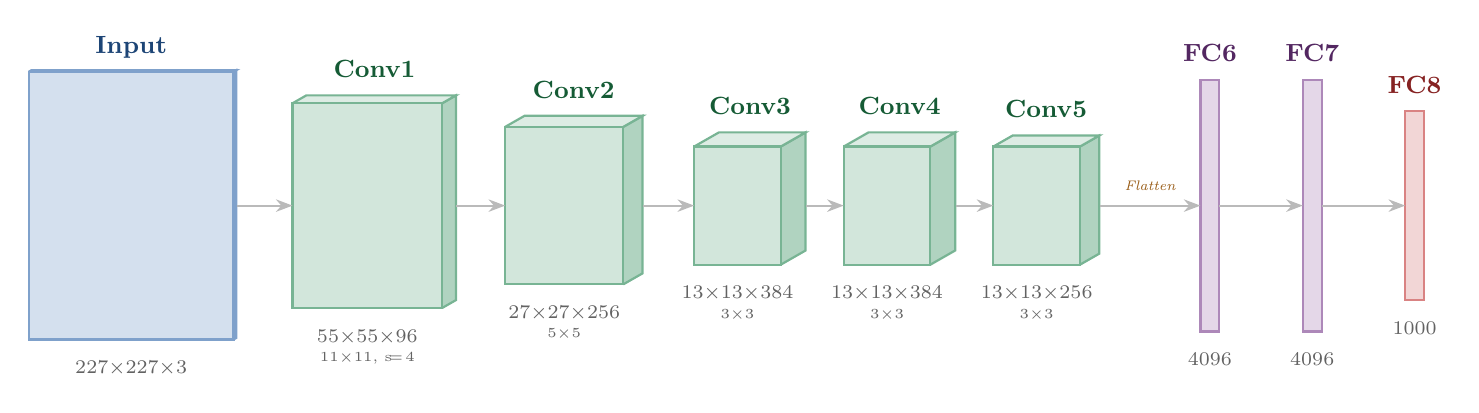
\begin{tikzpicture}[
    arrow/.style={-{Stealth[length=6pt]}, thick, draw=gdlgray!60},
    namelbl/.style={font=\small\bfseries, anchor=south},
    dimlbl/.style={font=\scriptsize, text=gdlgray!70!black, align=center, anchor=north}
]

% === Macro: cuboide pseudo-3D (capas convolucionales) ===
% #1=x, #2=y (centro cara frontal), #3=semi-ancho, #4=semi-alto, #5=profundidad, #6=color
\newcommand{\convblock}[6]{%
    \pgfmathsetmacro{\oX}{#5*0.35}%
    \pgfmathsetmacro{\oY}{#5*0.2}%
    % Cara derecha (más oscura, simula sombra)
    \fill[#6!35] ({#1+#3},{#2-#4}) -- ({#1+#3+\oX},{#2-#4+\oY})
        -- ({#1+#3+\oX},{#2+#4+\oY}) -- ({#1+#3},{#2+#4}) -- cycle;
    \draw[#6!60, thick] ({#1+#3},{#2-#4}) -- ({#1+#3+\oX},{#2-#4+\oY})
        -- ({#1+#3+\oX},{#2+#4+\oY}) -- ({#1+#3},{#2+#4});
    % Cara superior (más clara)
    \fill[#6!15] ({#1-#3},{#2+#4}) -- ({#1-#3+\oX},{#2+#4+\oY})
        -- ({#1+#3+\oX},{#2+#4+\oY}) -- ({#1+#3},{#2+#4}) -- cycle;
    \draw[#6!60, thick] ({#1-#3},{#2+#4}) -- ({#1-#3+\oX},{#2+#4+\oY})
        -- ({#1+#3+\oX},{#2+#4+\oY}) -- ({#1+#3},{#2+#4});
    % Cara frontal (relleno principal)
    \fill[#6!20] ({#1-#3},{#2-#4}) rectangle ({#1+#3},{#2+#4});
    \draw[#6!60, thick] ({#1-#3},{#2-#4}) rectangle ({#1+#3},{#2+#4});
}

% === Input (227x227x3) ===
\convblock{0}{0}{1.3}{1.7}{0.1}{gdlblue}
\node[namelbl, text=gdlblue!70!black] at (0, 1.74) {Input};
\node[dimlbl] at (0, -1.85) {$227{\times}227{\times}3$};

% === Conv1 (55x55x96, kernel 11x11, stride 4) ===
\convblock{3.0}{0}{0.95}{1.3}{0.5}{gdlgreen}
\node[namelbl, text=gdlgreen!70!black] at (3.09, 1.5) {Conv1};
\node[dimlbl] at (3.0, -1.45) {$55{\times}55{\times}96$\\[-1pt]{\tiny $11{\times}11$, s$\!=\!4$}};

% === Conv2 (27x27x256, kernel 5x5) ===
\convblock{5.5}{0}{0.75}{1.0}{0.7}{gdlgreen}
\node[namelbl, text=gdlgreen!70!black] at (5.62, 1.24) {Conv2};
\node[dimlbl] at (5.5, -1.15) {$27{\times}27{\times}256$\\[-1pt]{\tiny $5{\times}5$}};

% === Conv3 (13x13x384, kernel 3x3) ===
\convblock{7.7}{0}{0.55}{0.75}{0.9}{gdlgreen}
\node[namelbl, text=gdlgreen!70!black] at (7.86, 1.03) {Conv3};
\node[dimlbl] at (7.7, -0.9) {$13{\times}13{\times}384$\\[-1pt]{\tiny $3{\times}3$}};

% === Conv4 (13x13x384, kernel 3x3) ===
\convblock{9.6}{0}{0.55}{0.75}{0.9}{gdlgreen}
\node[namelbl, text=gdlgreen!70!black] at (9.76, 1.03) {Conv4};
\node[dimlbl] at (9.6, -0.9) {$13{\times}13{\times}384$\\[-1pt]{\tiny $3{\times}3$}};

% === Conv5 (13x13x256, kernel 3x3) ===
\convblock{11.5}{0}{0.55}{0.75}{0.7}{gdlgreen}
\node[namelbl, text=gdlgreen!70!black] at (11.62, 0.99) {Conv5};
\node[dimlbl] at (11.5, -0.9) {$13{\times}13{\times}256$\\[-1pt]{\tiny $3{\times}3$}};

% === FC6 (4096 neuronas) ===
\fill[gdlpurple!20] (13.58, -1.6) rectangle (13.82, 1.6);
\draw[gdlpurple!60, thick] (13.58, -1.6) rectangle (13.82, 1.6);
\node[namelbl, text=gdlpurple!70!black] at (13.7, 1.7) {FC6};
\node[dimlbl] at (13.7, -1.75) {4096};

% === FC7 (4096 neuronas) ===
\fill[gdlpurple!20] (14.88, -1.6) rectangle (15.12, 1.6);
\draw[gdlpurple!60, thick] (14.88, -1.6) rectangle (15.12, 1.6);
\node[namelbl, text=gdlpurple!70!black] at (15.0, 1.7) {FC7};
\node[dimlbl] at (15.0, -1.75) {4096};

% === FC8 / Salida (1000 clases) ===
\fill[gdlred!20] (16.18, -1.2) rectangle (16.42, 1.2);
\draw[gdlred!60, thick] (16.18, -1.2) rectangle (16.42, 1.2);
\node[namelbl, text=gdlred!70!black] at (16.3, 1.3) {FC8};
\node[dimlbl] at (16.3, -1.35) {1000};

% === Flechas de flujo entre capas ===
\draw[arrow] (1.34, 0) -- (2.05, 0);     % Input -> Conv1
\draw[arrow] (4.13, 0) -- (4.75, 0);     % Conv1 -> Conv2
\draw[arrow] (6.50, 0) -- (7.15, 0);     % Conv2 -> Conv3
\draw[arrow] (8.57, 0) -- (9.05, 0);     % Conv3 -> Conv4
\draw[arrow] (10.47, 0) -- (10.95, 0);   % Conv4 -> Conv5
\draw[arrow] (12.30, 0) -- (13.58, 0);   % Conv5 -> FC6 (flatten)
\draw[arrow] (13.82, 0) -- (14.88, 0);   % FC6 -> FC7
\draw[arrow] (15.12, 0) -- (16.18, 0);   % FC7 -> FC8

% === Anotación "Flatten" entre Conv5 y FC6 ===
\node[font=\tiny\itshape, text=gdlorange!70!black, above=2pt] at (12.94, 0) {Flatten};

\end{tikzpicture}
\end{document}
